\index{type!family of|(}%
\index{transport|(defstyle}%
Since \emph{dependently typed} functions are essential in type theory, we will also need a version of \cref{lem:map} for these.
However, this is not quite so simple to state, because if $f:\prd{x:A} B(x)$ and $p:x=y$, then $f(x):B(x)$ and $f(y):B(y)$ are elements of distinct types, so that \emph{a priori} we cannot even ask whether they are equal.
The missing ingredient is that $p$ itself gives us a way to relate the types $B(x)$ and $B(y)$.

We have already seen this in \autoref{sec:identity-types}, where we called it ``indiscernibility of identicals''.
\index{indiscernibility of identicals}%
We now introduce a different name and notation for it that we will use from now on.

\begin{lem}[Transport]\label{lem:transport}
  Suppose that $P$ is a type family over $A$ and that $p:\id[A]xy$.
  Then there is a function $\transf{p}:P(x)\to P(y)$.
\end{lem}

\begin{proof}[First proof]
  Let $D:\prd{x,y:A} (\id{x}{y}) \to \type$ be the type family defined by
  \[D(x,y,p)\defeq P(x)\to P(y).\]
  Then we have the function
  \begin{equation*}
    d\defeq\lam{x} \idfunc[P(x)]:\prd{x:A} D(x,x,\refl{x}),
  \end{equation*}
  so that the induction principle gives us $\indid{A}(D,d,x,y,p):P(x)\to P(y)$ for $p:x= y$, which we define to be $\transf p$.
\end{proof}

\begin{proof}[Second proof]
  By induction, it suffices to assume $p$ is $\refl x$.
  But in this case, we can take $\transf{(\refl x)}:P(x)\to P(x)$ to be the identity function.
\end{proof}

Sometimes, it is necessary to notate the type family $P$ in which the transport operation happens.
In this case, we may write
\[\transfib P p \blank : P(x) \to P(y).\]

Recall that a type family $P$ over a type $A$ can be seen as a property of elements of $A$, which holds at $x$ in $A$ if $P(x)$ is inhabited.
Then the transportation lemma says that $P$ respects equality, in the sense that if $x$ is equal to $y$, then $P(x)$ holds if and only if $P(y)$ holds.
In fact, we will see later on that if $x=y$ then actually $P(x)$ and $P(y)$ are \emph{equivalent}.

Topologically, the transportation lemma can be viewed as a ``path lifting'' operation in a fibration.
\index{fibration}%
\indexdef{total!space}%
We think of a type family $P:A\to \type$ as a \emph{fibration} with base space $A$, with $P(x)$ being the fiber over $x$, and with $\sm{x:A}P(x)$ being the \define{total space} of the fibration, with first projection $\sm{x:A}P(x)\to A$.
The defining property of a fibration is that given a path $p:x=y$ in the base space $A$ and a point $u:P(x)$ in the fiber over $x$, we may lift the path $p$ to a path in the total space starting at $u$ (and this lifting can be done continuously).
The point $\trans p u$ can be thought of as the other endpoint of this lifted path.
We can also define the path itself in type theory:

\begin{lem}[Path lifting property]\label{thm:path-lifting}
  \indexdef{path!lifting}%
  \indexdef{lifting!path}%
  Let $P:A\to\type$ be a type family over $A$ and assume we have $u:P(x)$ for some $x:A$.
  Then for any $p:x=y$, we have
  \begin{equation*}
    \mathsf{lift}(u,p):(x,u)=(y,\trans{p}{u})
  \end{equation*}
  in $\sm{x:A}P(x)$, such that $\ap{\proj1}{\mathsf{lift}(u,p)} = p$.
\end{lem}
\begin{proof}
  Left to the reader.
  We will prove a more general theorem in \cref{sec:compute-sigma}.
\end{proof}

In classical homotopy theory, a fibration is defined as a map for which there \emph{exist} liftings of paths; while in contrast, we have just shown that in type theory, every type family comes with a \emph{specified} ``path-lifting function''.
This accords with the philosophy of constructive mathematics, according to which we cannot show that something exists except by exhibiting it.
\index{continuity of functions in type theory@``continuity'' of functions in type theory}%
It also ensures automatically that the path liftings are chosen ``continuously'', since as we have seen, all functions in type theory are ``continuous''.

\begin{rmk}
  Although we may think of a type family $P:A\to \type$ as like a fibration, it is generally not a good idea to say things like ``the fibration $P:A\to\type$'', since this sounds like we are talking about a fibration with base $\type$ and total space $A$.
  To repeat, when a type family $P:A\to \type$ is regarded as a fibration, the base is $A$ and the total space is $\sm{x:A} P(x)$.

  We may also occasionally use other topological terminology when speaking about type families.
  For instance, we may refer to a dependent function $f:\prd{x:A} P(x)$ as a \define{section}
  \indexdef{section!of a type family}%
  of the fibration $P$, and we may say that something happens \define{fiberwise}
  \indexdef{fiberwise}%
  if it happens for each $P(x)$.
  For instance, a section $f:\prd{x:A} P(x)$ shows that $P$ is ``fiberwise inhabited''.
\end{rmk}

\index{function!dependent|(}
Now we can prove the dependent version of \cref{lem:map}.
The topological intuition is that given $f:\prd{x:A} P(x)$ and a path $p:\id[A]xy$, we ought to be able to apply $f$ to $p$ and obtain a path in the total space of $P$ which ``lies over'' $p$, as shown below.

\begin{center}
  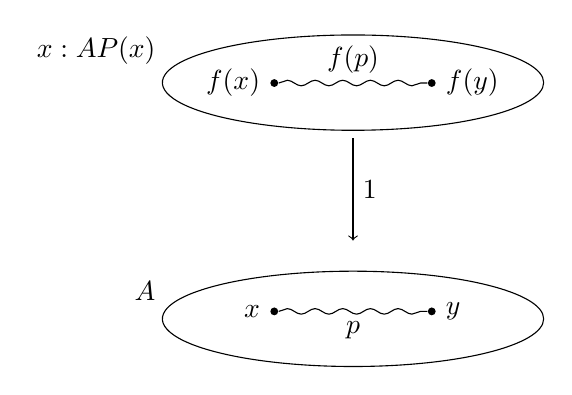
\begin{tikzpicture}[yscale=.5,xscale=2]
    \draw (0,0) arc (-90:170:8ex) node[anchor=south east] {$A$} arc (170:270:8ex);
    \draw (0,6) arc (-90:170:8ex) node[anchor=south east] {$\sm{x:A} P(x)$} arc (170:270:8ex);
    \draw[->] (0,5.8) -- node[auto] {$\proj1$} (0,3.2);
    \node[circle,fill,inner sep=1pt,label=left:{$x$}] (b1) at (-.5,1.4) {};
    \node[circle,fill,inner sep=1pt,label=right:{$y$}] (b2) at (.5,1.4) {};
    \draw[decorate,decoration={snake,amplitude=1}] (b1) -- node[auto,swap] {$p$} (b2);
    \node[circle,fill,inner sep=1pt,label=left:{$f(x)$}] (b1) at (-.5,7.2) {};
    \node[circle,fill,inner sep=1pt,label=right:{$f(y)$}] (b2) at (.5,7.2) {};
    \draw[decorate,decoration={snake,amplitude=1}] (b1) -- node[auto] {$f(p)$} (b2);
  \end{tikzpicture}
\end{center}

We \emph{can} obtain such a thing from \cref{lem:map}.
Given $f:\prd{x:A} P(x)$, we can define a non-dependent function $f':A\to \sm{x:A} P(x)$ by setting $f'(x)\defeq (x,f(x))$, and then consider $\ap{f'}{p} : f'(x) = f'(y)$.
Since $\proj1 \circ f' \jdeq \idfunc[A]$, by \cref{lem:ap-functor} we have $\ap{\proj1}{\ap{f'}{p}} = p$; thus $\ap{f'}{p}$ does ``lie over'' $p$ in this sense.
However, it is not obvious from the \emph{type} of $\ap{f'}{p}$ that it lies over any specific path in $A$ (in this case, $p$), which is sometimes important.

The solution is to use the transport lemma.
By \cref{thm:path-lifting} we have a canonical path $\mathsf{lift}(u,p)$ from $(x,u)$ to $(y,\trans p u)$ which lies over $p$.
Thus, any path from $u:P(x)$ to $v:P(y)$ lying over $p$ should factor through $\mathsf{lift}(u,p)$, essentially uniquely, by a path from $\trans p u$ to $v$ lying entirely in the fiber $P(y)$.
Thus, up to equivalence, it makes sense to define ``a path from $u$ to $v$ lying over $p:x=y$'' to mean a path $\trans p u = v$ in $P(y)$.
And, indeed, we can show that dependent functions produce such paths.

\begin{lem}[Dependent map]\label{lem:mapdep}
  \indexdef{application!of dependent function to a path}%
  \indexdef{path!application of a dependent function to}%
  \indexdef{function!dependent!application to a path of}%
  \indexdef{action!of a dependent function on a path}%
  Suppose $f:\prd{x: A} P(x)$; then we have a map
  \[\apdfunc f : \prd{p:x=y}\big(\id[P(y)]{\trans p{f(x)}}{f(y)}\big).\]
\end{lem}

\begin{proof}[First proof]
  Let $D:\prd{x,y:A} (\id{x}{y}) \to \type$ be the type family defined by
  \begin{equation*}
    D(x,y,p)\defeq \trans p {f(x)}= f(y).
  \end{equation*}
  Then $D(x,x,\refl{x})$ is $\trans{(\refl{x})}{f(x)}= f(x)$.
  But since $\trans{(\refl{x})}{f(x)}\jdeq f(x)$, we get that $D(x,x,\refl{x})\jdeq (f(x)= f(x))$.
  Thus, we find the function
  \begin{equation*}
    d\defeq\lam{x} \refl{f(x)}:\prd{x:A} D(x,x,\refl{x})
  \end{equation*}
  and now path induction gives us $\apdfunc f(p):\trans p{f(x)}= f(y)$ for each $p:x= y$.
\end{proof}

\begin{proof}[Second proof]
  By induction, it suffices to assume $p$ is $\refl x$.
  But in this case, the desired equation is $\trans{(\refl{x})}{f(x)}= f(x)$, which holds judgmentally.
\end{proof}

We will refer generally to paths which ``lie over other paths'' in this sense as \emph{dependent paths}.
\indexsee{dependent!path}{path, dependent}%
\index{path!dependent}%
They will play an increasingly important role starting in \cref{cha:hits}.
In \cref{sec:computational} we will see that for a few particular kinds of type families, there are equivalent ways to represent the notion of dependent paths that are sometimes more convenient.

Now recall from \cref{sec:pi-types} that a non-dependently typed function $f:A\to B$ is just the special case of a dependently typed function $f:\prd{x:A} P(x)$ when $P$ is a constant type family, $P(x) \defeq B$.
In this case, $\apdfunc{f}$ and $\apfunc{f}$ are closely related, because of the following lemma:

\begin{lem}\label{thm:trans-trivial}
  If $P:A\to\type$ is defined by $P(x) \defeq B$ for a fixed $B:\type$, then for any $x,y:A$ and $p:x=y$ and $b:B$ we have a path
  \[ \transconst Bpb : \transfib P p b = b. \]
\end{lem}
\begin{proof}[First proof]
  Fix a $b:B$, and let $D:\prd{x,y:A} (\id{x}{y}) \to \type$ be the type family defined by
  \[ D(x,y,p) \defeq (\transfib P p b = b). \]
  Then $D(x,x,\refl x)$ is $(\transfib P{\refl{x}}{b} = b)$, which is judgmentally equal to $(b=b)$ by the computation rule for transporting.
  Thus, we have the function
  \[ d \defeq \lam{x} \refl{b} : \prd{x:A} D(x,x,\refl x). \]
  Now path induction gives us an element of
  \narrowequation{
    \prd{x,y:A}{p:x=y}(\transfib P p b = b),}
  as desired.
\end{proof}
\begin{proof}[Second proof]
  By induction, it suffices to assume $y$ is $x$ and $p$ is $\refl x$.
  But $\transfib P {\refl x} b \jdeq b$, so in this case what we have to prove is $b=b$, and we have $\refl{b}$ for this.
\end{proof}

Thus, for any $x,y:A$ and $p:x=y$ and $f:A\to B$, by concatenating with $\transconst Bp{f(x)}$ and its inverse, respectively, we obtain functions
\begin{align}
  \big(f(x) = f(y)\big) &\to \big(\trans{p}{f(x)} = f(y)\big)\label{eq:ap-to-apd}
  \qquad\text{and} \\
  \big(\trans{p}{f(x)} = f(y)\big) &\to \big(f(x) = f(y)\big).\label{eq:apd-to-ap}
\end{align}
In fact, these functions are inverse equivalences (in the sense to be introduced in \cref{sec:basics-equivalences}), and they relate $\apfunc f (p)$  to $\apdfunc f (p)$.

\begin{lem}\label{thm:apd-const}
  For $f:A\to B$ and $p:\id[A]xy$, we have
  \[ \apdfunc f(p) = \transconst B p{f(x)} \ct \apfunc f (p). \]
\end{lem}
\begin{proof}[First proof]
  Let $D:\prd{x,y:A} (\id xy) \to \type$ be the type family defined by
  \[ D(x,y,p) \defeq \big(\apdfunc f (p) = \transconst Bp{f(x)} \ct \apfunc f (p)\big). \]
  Thus, we have
  \[D(x,x,\refl x) \jdeq \big(\apdfunc f (\refl x) = \transconst B{\refl x}{f(x)} \ct \apfunc f ({\refl x})\big).\]
  But by definition, all three paths appearing in this type are $\refl{f(x)}$, so we have
  \[ \refl{\refl{f(x)}} : D(x,x,\refl x). \]
  Thus, path induction gives us an element of $\prd{x,y:A}{p:x=y} D(x,y,p)$, which is what we wanted.
\end{proof}
\begin{proof}[Second proof]
  By induction, it suffices to assume $y$ is $x$ and $p$ is $\refl x$.
  In this case, what we have to prove is $\refl{f(x)} = \refl{f(x)} \ct \refl{f(x)}$, which is true judgmentally.
\end{proof}

Because the types of $\apdfunc{f}$ and $\apfunc{f}$ are different, it is often clearer to use different notations for them.
% We may sometimes use a notation $\apd f p$ for $\apdfunc{f}(p)$, which is similar to the notation $\ap f p$ for $\apfunc{f}(p)$.

\index{function!dependent|)}%

At this point, we hope the reader is starting to get a feel for proofs by induction on identity types.
From now on we stop giving both styles of proofs, allowing ourselves to use whatever is most clear and convenient (and often the second, more concise one).
Here are a few other useful lemmas about transport; we leave it to the reader to give the proofs (in either style).

\begin{lem}\label{thm:transport-concat}
  Given $P:A\to\type$ with $p:\id[A]xy$ and $q:\id[A]yz$ while $u:P(x)$, we have
  \[ \trans{q}{\trans{p}{u}} = \trans{(p\ct q)}{u}. \]
\end{lem}

\begin{lem}\label{thm:transport-compose}
  For a function $f:A\to B$ and a type family $P:B\to\type$, and any $p:\id[A]xy$ and $u:P(f(x))$, we have
  \[ \transfib{P\circ f}{p}{u} = \transfib{P}{\apfunc f(p)}{u}. \]
\end{lem}

\begin{lem}\label{thm:ap-transport}
  For $P,Q:A\to \type$ and a family of functions $f:\prd{x:A} P(x)\to Q(x)$, and any $p:\id[A]xy$ and $u:P(x)$, we have
  \[ \transfib{Q}{p}{f_x(u)} = f_y(\transfib{P}{p}{u}). \]
\end{lem}

\index{type!family of|)}%
\index{transport|)}